\documentclass{report}

\usepackage{textcomp}
\usepackage{graphicx}
\usepackage{fancyhdr}
\usepackage{subcaption}
\usepackage{multicol}
\usepackage{outlines}
%===================================
\newcommand{\classinfo}{{\bf RHEL Labs \\ Week 06}\\{\it CIT 217}\\{Chaz Davis}}
\newcommand{\semester}{BCTC \\ Spring 2020}
%===================================
\newcommand{\mysection}[1]{\section*{#1}}
\newcommand{\mysubsection}[2]{\textbf{\romannumeral #1) #2}}
%===================================
\setlength{\headheight}{15.2pt}
\pagestyle{fancy}
\fancyhf{}
\lhead{ \fancyplain{}{Chaz Davis} }
\rhead{ \fancyplain{}{\today} }
\cfoot{ \fancyplain{}{\thepage} }
\renewcommand{\headrulewidth}{0.5pt}
\renewcommand{\footrulewidth}{0pt}

%===================================
\title{\classinfo}
\author{\semester}
\date{\today}

%===================================

\begin{document}

\maketitle

%===================================
\mysection{\textbf{Chapter 10}}

\mysubsection{1}{Use the logger command to manually enter a message with your 
first and last name into syslog. Provide the last 5 lines of the log file 
containing your message.}
I logged into the student server, opened terminal. Using
the {\scriptsize{\verb$su -$}\normalsize} command I setup system-debug and
restarted systemctl. Then under the Student user, I sent my name to the syslog.
as seen in Fig.~\ref{Ch10}\subref{Ch10Log}.


\noindent\mysubsection{2}{Use the journalctl command to find all the priority err entries since 5 days ago. Provide the Output.}
\\I ran {\scriptsize{\verb$date -d '5 days ago'$}\normalsize} to
get the date for 5 days ago. I then ran the 
command {\scriptsize{\verb$journalctl -p err --since "2020-02-18"$}\normalsize} 
by passing the -p err flag i was able to get just the errors logged  and the
--since flag gave me all logs since a certain date 
as seen in Fig.~\ref{Ch10}\subref{Ch10ctl}.


\begin{figure}[!b]\centering
\subfloat[Logger command output]{\label{Ch10Log}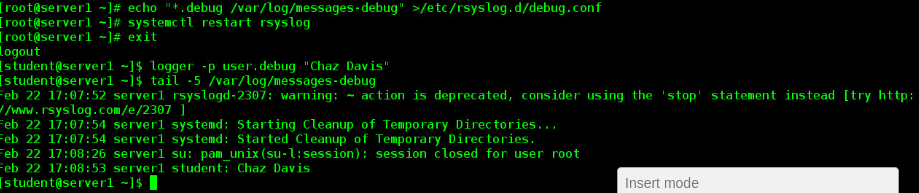
\includegraphics[width=.75\linewidth]{Figures/2020-02-22-171028_919x193_scrot.png}}\par
\subfloat[Journalctl priority Err
output]{\label{Ch10ctl}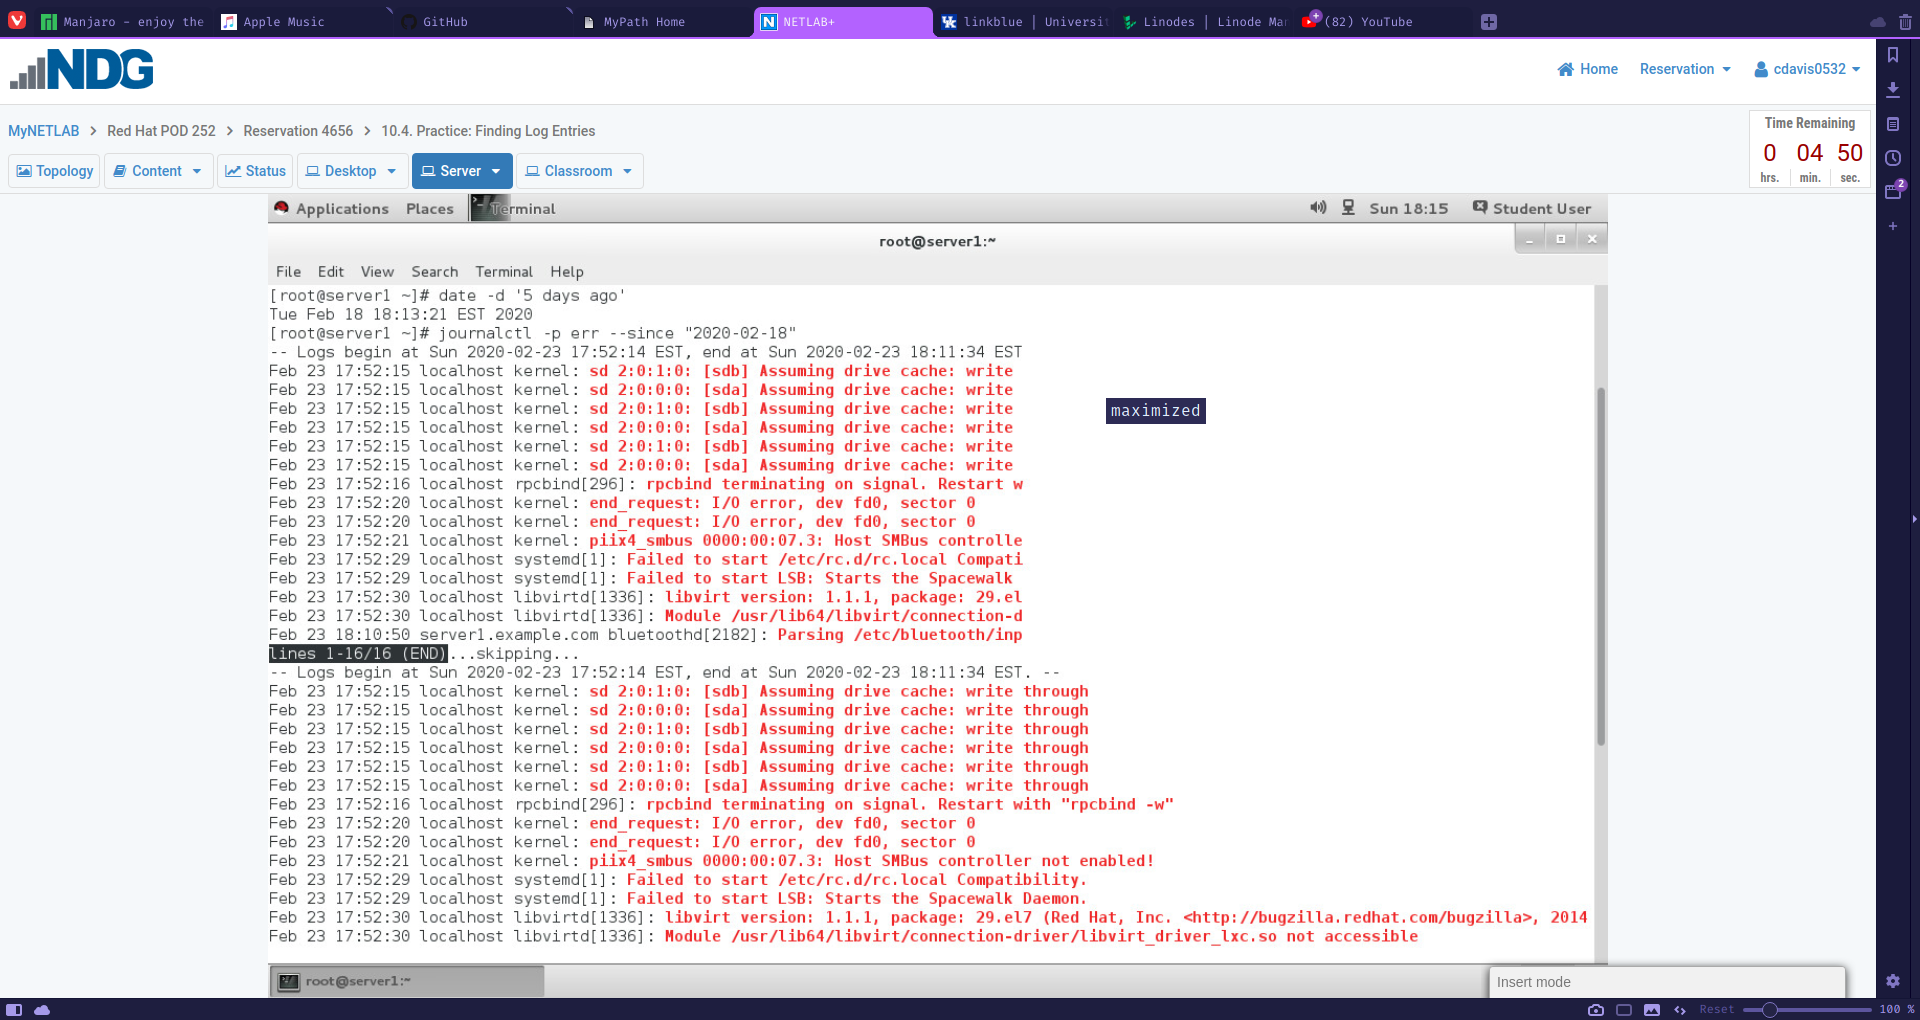
\includegraphics[width=.75\linewidth]{Figures/2020-02-23-181510_1920x1020_scrot.png}}\par
\caption{Chapter 10 screenshots}
\label{Ch10}
\end{figure}


\clearpage

%===================================
\mysection{\textbf{Chapter 11}}


\mysubsection{1}{Provide the output of all open ports on the machine}
\\To show all the open ports I
ran {\scriptsize{\verb$ss -ltn$}\normalsize} See
Fig.~\ref{Ch11}\subref{Ch11ports}.


\noindent\mysubsection{2}{Provide the output of the network address, netmask, and
routing table of the Desktop virtual machine.}
\\For the network address output I 
ran {\scriptsize{\verb$nmcli con show active$}\normalsize} see
Fig.~\ref{Ch11}\subref{Ch11Netadd}
\\For the routing table I ran {\scriptsize{\verb$ip route$}\normalsize} See
Fig.~\ref{Ch11}\subref{Ch11Rtable}.

\noindent\mysubsection{3}{Use the ping command to send exactly 5 ping packets to the
address 8.8.8.8 and provide the output. Was your ping successful or
unsuccessful?}
\\I ran {\scriptsize{\verb$ping -c5 8.8.8.8$}\normalsize}
Fig.~\ref{Ch11}\subref{Ch11Ping}.


\begin{figure}[!b]\centering
\subfloat[All open ports]{\label{Ch11ports}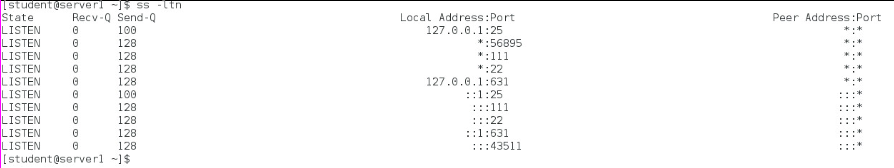
\includegraphics[width=.65\linewidth]{Figures/2020-02-23-200617_894x168_scrot.png}}\par
\subfloat[Network address]{\label{Ch11Netadd}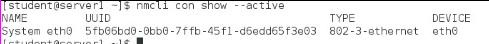
\includegraphics[width=.50\linewidth]{Figures/2020-02-23-201013_489x44_scrot.png}}\hfill
\subfloat[netmask]{\label{Ch11Netmask}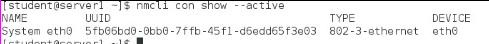
\includegraphics[width=.50\linewidth]{Figures/2020-02-23-201013_489x44_scrot.png}}\par
\subfloat[routing table]{\label{Ch11Rtable}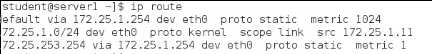
\includegraphics[width=.50\linewidth]{Figures/2020-02-23-201031_432x54_scrot.png}}\hfill
\subfloat[ping 8.8.8.8]{\label{Ch11Ping}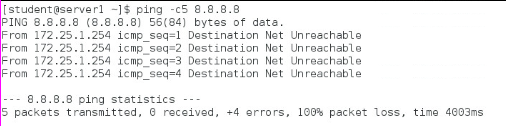
\includegraphics[width=.50\linewidth]{Figures/2020-02-23-203537_506x126_scrot.png}}\par
\caption{Chapter 11 screenshots}
\label{Ch11}
\end{figure}


\clearpage


%===================================
\mysection{\textbf{Chapter 12}}

\mysubsection{1}{Create a gzip-compressed tar file of the /var/log/ directory named 
log.tar.gz. Use the tar cammond to provide the details of the log.tar.gz tarball.}
I ran {\scriptsize{\verb$tar czf /tmp/log.tar.gz /var/log$}\normalsize} 
see Fig.~\ref{Ch12}\subref{Ch12log}
I then ran {\scriptsize{\verb$tar -tvf /tmp/log.tar.gz$}\normalsize} to list
the files. 
see Fig.~\ref{Ch12}\subref{Ch12linfo}
\hfill\break

\noindent\mysubsection{2}{Use the scp command to copy the log.tar.gz file from the
Desktop VM to the Server VM. Provide a detailed
list of the directory on the Server VM where the file was copied to.}
\\I ran {\scriptsize{\verb$ssh root@server1$}\normalsize} to log into the
server over ssh and establish a connection. The, exited. I then created the tarball as I did in step 1 above. Next,
I used the command 
{\scriptsize{\verb$scp /tmp/log.tar.gz server1:/home/student/$}\normalsize} 
see Fig.~\ref{Ch12}\subref{Ch12scpsend}
once on Server1 I went to the home directory for student and ran the commands
as above to list the files in the archive.
see Fig.~\ref{Ch12}\subref{Ch12scplist}



\begin{figure}[!b]\centering
\subfloat[Gzip log]{\label{Ch12log}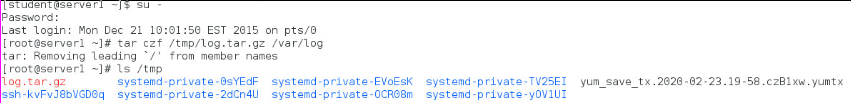
\includegraphics[width=.65\linewidth]{Figures/2020-02-23-205633_851x103_scrot.png}}\hfill
\subfloat[Gzip log output]{\label{Ch12linfo}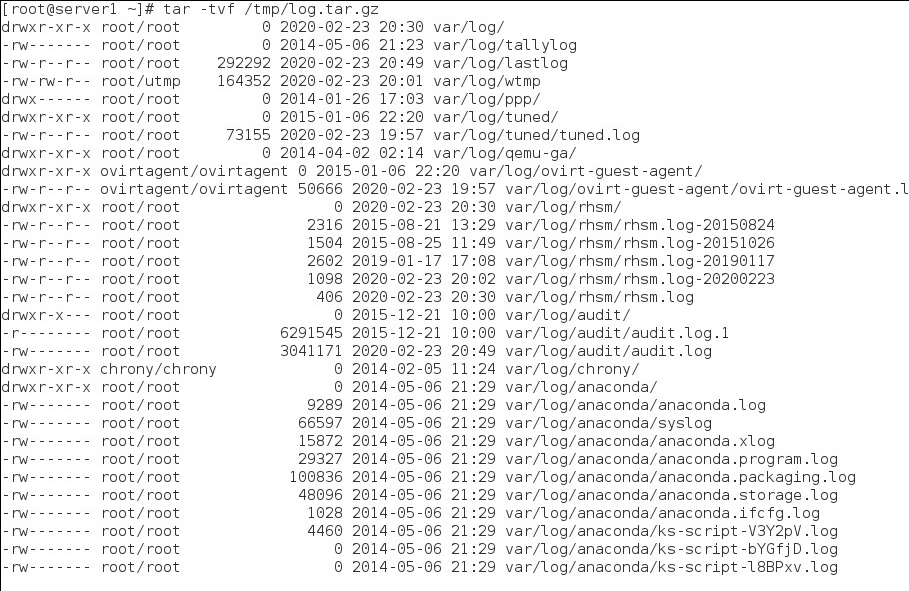
\includegraphics[width=.65\linewidth]{Figures/2020-02-23-205801_909x591_scrot.png}}\par
\subfloat[Sending the tarball over scp]{\label{Ch12scpsend}
\includegraphics[width=.65\linewidth]{Figures/2020-02-23-211326_492x27_scrot.png}}\hfill
\subfloat[List of the tar.gz file after scp]{\label{Ch12scplist}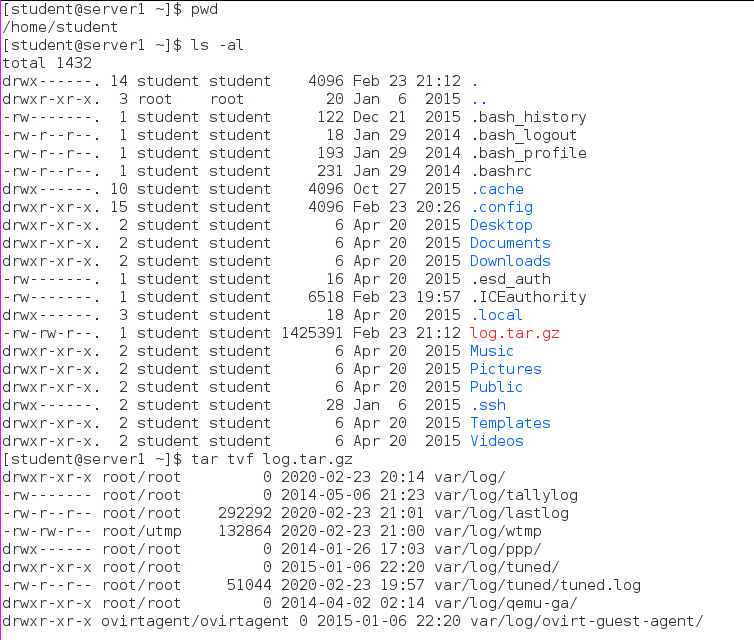
\includegraphics[width=.65\linewidth]{Figures/2020-02-23-211440_754x640_scrot.png}}\hfill
\caption{Chapter 12 Screenshots}
\label{Ch12}
\end{figure}


%===================================

\end{document}
